\input{notes.tex}

\usetikzlibrary{arrows}
\iftoggle{dualscreen}{\setbeameroption{show notes on second screen=right}}{}


\begin{document}

\section{Lecture 12}
\subsection{Preamble}


\subsection{Inverting Laplace Transforms}
\slide[Recall: Laplace Transforms]{
Laplace Transform as a mapping from time-domain to s-domain: \algn{\mathcal{L}: f(t) &\rightarrow F(s)\\
y(t) &\mapsto Y(s) = \intop_0^\infty e^{-st}y(t)dt}
How can we go back to the time domain?
\vfill
\student{
\centerline{This mapping is bijective for most practical cases}\vfill
\ex{time-domain: $y(t)=\frac12 \quad \Rightarrow \quad $ s-domain: $Y(s)=\frac1{2s}$}\vfill
We can also reverse the arrow...\vfill
s-domain: $H(s)=\frac1{2s}  \quad \Rightarrow \quad $time-domain: $h(t)=\frac12$

}
\vfill

}


\slide[Bijectivity of the Laplace Transform \hfill \small(not true for all functions)]{\centerline{
\resizebox{.75\textwidth}{!}{
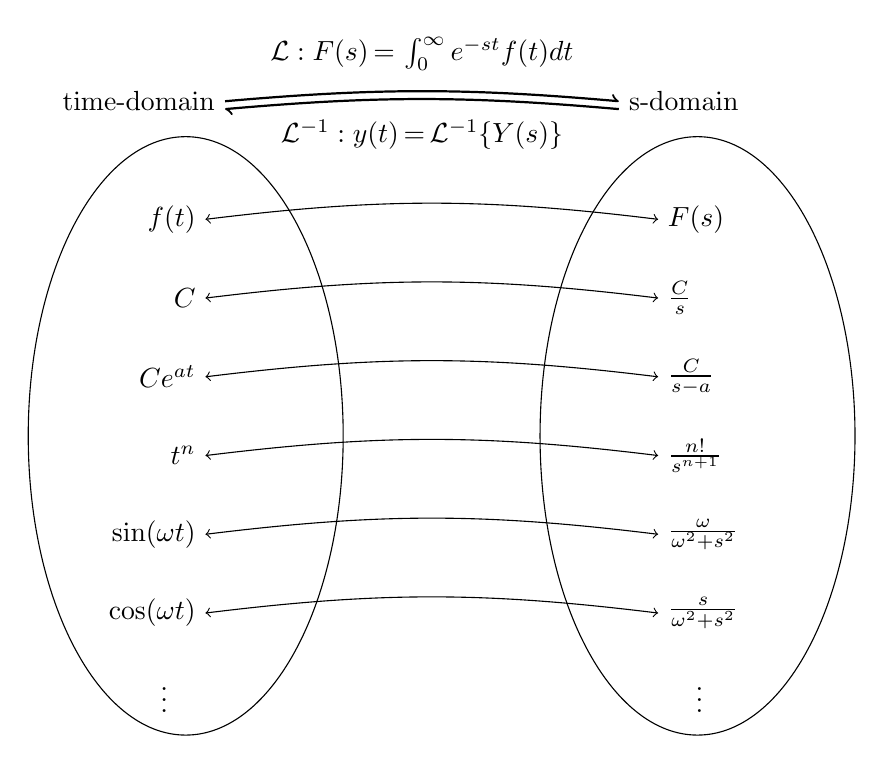
\begin{tikzpicture}
\draw[-left to, thick, ] (1,0) node[align=center, left]{time-domain} to [out=5,in=175]   node[label= above:$\mathcal{L} : F(s)   {\,\displaystyle =\,} \intop_0^\infty e^{-st} f(t) dt$]  {} (6,0) node[align=center, right]{s-domain};
\draw[-left to, thick]   (6,-0.1)  to [out=175,in=5]  node[label= below:$\mathcal{L}^{-1}: y(t)  {\,\displaystyle =\,} \mathcal{L}^{-1}\{Y(s)\} $] {}(1,-0.1) ;
\draw (0.5,-4.25) ellipse (2cm and 3.8cm);
\draw (7,-4.25) ellipse (2cm and 3.8cm);
\draw[<->] (0.75,-1.5) node[left]{$f(t)$} to [out=7,in=173]  (6.5,-1.5) node[right]{$F(s)$} ;

\foreach \y\Y\i in
 { C/\frac{C}{s}/2, 
Ce^{at}/\frac{C}{s-a}/3, 
t^n/\frac{n!}{s^{n+1}}/4,
\sin(\omega t)/\frac{\omega}{\omega^2+s^2}/5 ,
\cos(\omega t)/\frac{s}{\omega^2+s^2}/6 }{
\draw[<->] (0.75,-\i-.5) node[left]{$\y$}  to [out=7,in=173]  (6.5,-\i-.5) node[right]{$\Y$} ;

}

\draw (0.75,-7.5) node[left]{$\vdots\quad$} ;
\draw (6.5,-7.5) node[right]{$\quad\vdots$} ;
\end{tikzpicture}}
}

}

\slide{\ex{Suppose $Y(s)=\frac{1}{s+6}$, find $y(t)$.}
\student{\algn{ Y(s) &=  \frac{C}{s-a} &C&=1,\quad a=-6\\
y(t) &= \lapinv{\frac{1}{s+6}} = e^{-6t}
}}\vfill
\ex{Suppose $G(s)=\frac{12}{s^2+16}$, find g(t).}
\student{\algn{ G(s) &=  C \frac{\omega}{s+\omega^2} &C&=3,\quad \omega=4\\
g(t) &= \lapinv{\frac{12}{s^2+16}} = 3\sin(4t)
}}
\vfill
}

\slide{
\ex{Suppose $Y(s)=\frac{s-1}{9+s^2}$, find $y(t)$}
\vfill
\student{
\algn{
Y(s) &=\frac{-1}{9+s^2} +\frac{s}{9+s^2}\\
&=A \underbrace{\frac{\omega}{s^2+\omega^2}}_{\lap{\sin \omega t}} + \underbrace{\frac{s}{s^2+\omega^2}}_{\lap{\cos \omega t}} &&\omega=3\\\\
&=A \frac{3}{s^2+9} +\frac{s}{s^2+9} && A\cdot3=-1\\
Y(s)&=\frac{-1}{3} \frac{3}{s^2+9} +\frac{s}{s^2+9} &&A=-\frac13\\
y(t)&=-\frac13 \sin(3t)+\cos(3t)
}
}
}

\slide{
\ex{Suppose $H(s)=\frac{4}{s^2+6s+25}$, find h(t).}\vfill
\student{
Kind of looks like previous example, but denominator is not quite right.
\\~\\
Try completing the square.  \[as^2+bs+c = a(s+d)^2 + e \qquad \larray{d=\frac{b}{2a} \\ e = c-\frac{b^2}{4a}}\]
\algn{ H(s) &= \frac{4}{s^2+6s+25} & &\larray{d=\frac{6}{2}=3 \\ e = 25-\frac{36}{4} = 16}\\
&=\frac{4}{(s+3)^2+16}}
\vfill
Looks similar to LT of $sin(4t)$, but $s$ is shifted.
}
\vfill

}

\slide[First Shift Theorem: Multiplication by $e^{a t}$]{
\student{
\algn{\lap{e^{a t}f(t)}&=\lapint{e^{a t}f(t)}\\
&=\int_0^\infty e^{-(s-a)t}f(t)dt&\text{let }\tilde{s} = s-a\\
\int_0^\infty e^{\tilde{s}t}f(t)dt  &=F(\tilde{s})\\
\Aboxed{\lap{e^{a t}f(t)} &= F(s-a)}}
\vfill
\uline{Take home:}\vfill
If you  recognize something in the $s$-domain but with $s \to s-a$, multiply by $e^{at}$ in the time domain.\vfill
}

}

\slide{
\ex{Suppose $H(s)=\frac{4}{(s+3)^2+16}$, find h(t).}\vfill
\student{
\algn{H(s) &= \frac{4}{s^2+16}\evalat{ s=s+3 }{} \quad =\quad   \lap{\sin(4t)} \evalat{ s=s+3 }{}\\\\
h(t) &= e^{-3t} \lapinv{\frac{4}{s^2+16}} = e^{-3t} \sin(4t)
}
\vfill

}
\vfill

}



\slide{
\ex{Suppose $Y(s) = \frac{3}{s(s+6)}+\frac{2}{s+6}$, find $y(t)$.}
\student{
\algn{Y(s) = \underbrace{\frac{3}{s(s+6)}}_{\lap{???}} +2 \lap{e^{-6t}} \intertext{Partial fraction decomposition}
\frac{3}{s(s+6)}&=\frac{A}{s}+\frac{B}{s+6}\intertext{multiply by denominator}
3&=A (s+6)+B\cdot s\\
&=6A + (A+B)s\\
\intertext{True for all $s$ $\Rightarrow$ coefficients must match}
\text{\uline{constant terms}:}\quad 3&=6A &&A=\frac12\\
\text{\uline{$s$ terms}:}\quad 0&=A+B &&B=-A=-\frac12\\\\
Y(s) = \frac{1}{2s}-\frac{1}{2(s+6)} +\frac{y_0}{s+6}&=\frac{1}{2s}+\paren{y_0-\frac12}\frac{1}{s+6}
}

}
}

\slide{

\student{
\algn{\ucover{Y(s)}&\ucover{=\frac{1}{2s}-\frac12  \frac{1}{s+6} + \frac{2}{s+6}}\\
&=\frac{1}{2s}+\frac32  \frac{1}{s+6}  \\
&=\lap{\frac12} + \frac32 \lap{e^{-6t}}\\\\
y(t)&=\frac{1}{2}+\frac32 e^{-6t}}
}\vfill
}



\slide{\ex{Suppose $Y(s) = \frac{s+4}{(s-4)^2(s+1)}$, find $y(t)$} 
\student{
\algn{ \frac{s+4}{(s-4)^2(s+1)} &= \frac{A}{(s-4)^2} +  \frac{B}{(s-4)} +  \frac{C}{(s+1)}\\
s+4 &= A(s+1)+B\underbrace{(s-4)(s+1)}_{s^2-3s-4} + C \underbrace{(s-4)^2}_{s^2-8s+16}\\
s+4  &=(B+C)s^2+(A-3B-8C)s + A-4B+16C \intertext{match coeffiecients}
\uline{s^2:}\quad B+C&=0 \quad \Rightarrow B=-C\qquad \boxed{B=-\frac{3}{25}}\\
\uline{s:}\quad A-3B-8C&=1\\
A-5C&=1  \quad \Rightarrow A=1+5C \qquad \boxed{A=\frac{40}{25}}\\
\uline{s^0:}A-4B+16C&=4\\
1+25C&=4  \Rightarrow C=\frac{3}{25}\\
}
}

}
\slide{
\[Y(s) = \frac{40}{25}\student{\underbrace{\ucover{\frac{1}{(s-4)^2}}}_{\lap{t}\evalat{s=s-4}{}}} - \frac{3}{25}\student{\underbrace{\ucover{\frac{1}{(s-4)}}}_{\lap{e^{4t}}}} + \frac{3}{25}\student{\underbrace{\ucover{\frac{1}{(s+1)}}}_{\lap{e^{-t}}}} \] 
\student{\algn{y(t) &= \frac{40}{25} e^{4t}\lapinv{\frac{1}{s^2}} -  \frac{3}{25} e^{4t} +  \frac{3}{25} e^{-t}\\
&=\underbrace{ \frac{40}{25} te^{4t}}_{y_p} -\underbrace{  \frac{3}{25} e^{4t} +  \frac{3}{25} e^{-t}}_{y_h}}\vfill
Next lecture, we learn how to find Y(s) from an ODE.
}
}

\slide{\ex{Suppose $Y(s) = \frac{s-4}{((s+3)^2+16)(s+4)}$, find $y(t)$} 
\student{
\algn{
\frac{s-4}{((s+3)^2+16)(s+4)} &= \frac{As+B}{(s+3)^2+16} + \frac{C}{s+4}\\
s-4&= (As+B)(s+4) + C (s^2+6s+25)\\
s-4&=(A+C)s^2+(4A+B+6C)s+4B+25C\intertext{match coeffiecients}
\uline{s^2:}\quad A+C&=0 \quad \Rightarrow A=-C\qquad \boxed{A=\frac{8}{17}}\\
\uline{s:}\quad4A+B+6C&=1\\
B+2C&=1  \quad \Rightarrow B=1-2C \qquad \boxed{B=\frac{33}{17}}\\
\uline{s^0:}\quad4B+25C&=-4\\
4+17C&=-4  \Rightarrow \boxed{C=\frac{-8}{17}} \\
}}
}
\slide{
\student{
\algn{Y(s)&=\frac{8}{17}\underbrace{\frac{s}{(s+3)^2+16}}_{???} + \frac{33}{17}\underbrace{\frac{1}{(s+3)^2+16}}_{\frac14 \lap{e^{-3t}\sin(4t)}} - \frac{8}{17} \underbrace{\frac{1}{s+4}}_{\lap{e^{-4t}}}\\
&=\frac{8}{17}\Bigg[\underbrace{\frac{s+3}{(s+3)^2+16}}_{\lap{e^{-3t} \cos(4t)}}-\underbrace{\frac{3}{(s+3)^2+16}}_{\frac14 \lap{e^{-3t}\sin(4t)}} \Bigg]
+ \frac{33}{17}\frac{1}{(s+3)^2+16} \\& \phantom{=}- \frac{8}{17} \frac{1}{s+4}\\\\
y(t)& = \underbrace{e^{-3t} \left( \frac{8}{17} \cos(4t) +\frac{9}{68} \sin(4t) \right) }_{y_h}- \underbrace{\frac{8}{17} e^{-4t}}_{y_p}}
\vfill
Next lecture, we learn how to find Y(s) from an ODE.}
}

\slide[Summary: Inverting the Laplace transform of a function]{\vspace{-1em}
\ex{$Y(s) = \frac{s+4}{(s-4)^2(s+1)}$}\vfill 
\enum{
\item Do some algebra to get a sum of  "easy" terms 
\subitem{partial fraction decomposition \item completing the square}\vfill 
\centerline{\ex{$ Y(s) =   \frac85 \frac{1}{(s-4)^2}  - \frac15  \frac{1}{(s-4)} + \frac15 \frac{1}{(s+1)} $ }}\vfill
\item Transform back from $Y(s)$ to $y(t)$ using Laplace transform tables \subitem{Tackle each term in the sum individually. \item Go slowly when applying shift theorems}\vfill
\ex{~}\vspace{-2em}
\algn{y(t) &= \frac85 e^{4t}\lapinv{\frac{1}{s^2}} - \frac15 e^{4t} + \frac15 e^{-t}\\
&=\frac85 te^{4t} -\frac15 e^{4t} + \frac15 e^{-t}}
}
}


\end{document}